%!Mode::"UTF-8"
\documentclass[12pt]{article}

% 页面设置
\usepackage{geometry}
\geometry{left=2.5cm, right=2.5cm, top=2.5cm, bottom=2.5cm}
\usepackage{graphicx}
\usepackage{ctex}
\usepackage{fontspec}
\usepackage{setspace}

%高亮使用的颜色
\usepackage{xcolor}  	
\definecolor{commentcolor}{RGB}{0,121,121}
\definecolor{stringcolor}{RGB}{190,49,49}
\definecolor{keywordcolor}{RGB}{0,128,0}

% 代码设置
\usepackage{listings}
\usepackage{color}
\setmonofont{Consolas}
\definecolor{listing}{gray}{0.97}
\lstset{
	backgroundcolor=\color{listing},
	basicstyle=\footnotesize,
	commentstyle=\color{commentcolor},	%注释颜色
	keywordstyle=\color{keywordcolor}\textbf,	%关键词颜色
	stringstyle=\color{stringcolor},
	numbers=left,
	numberstyle=\footnotesize,
	stepnumber=1,
	aboveskip={0.5\baselineskip},
	belowskip={0.5\baselineskip},
	columns=fullflexible,
	breaklines=true,
	breakatwhitespace=true,
	frame=single,
	basicstyle=\ttfamily,
	numberstyle=\ttfamily,
	tabsize=3
}

% 字体设置
\setmainfont{Times New Roman}
\setCJKmainfont{SimSun}
\setCJKsansfont{SimHei}
\usepackage[version=4]{mhchem}
\usepackage{mathtools}
\usepackage{diffcoeff}

% 表格设置
\usepackage{makecell}
\newcommand{\addcell}[2][4]{\makecell{\zihao{#1}\textsf{#2}}}
\usepackage{titlesec}
\usepackage{booktabs}
\usepackage{tabularx}

% 设置图注、表注
\usepackage{caption}
\usepackage{bicaption}
\captionsetup{labelsep=quad, font={small, bf}, skip=2pt}
\DeclareCaptionOption{english}[]{
    \renewcommand\figurename{Fig.}
    \renewcommand\tablename{Table}
}
\captionsetup[bi-second]{english}

% 设置页眉
\usepackage{fancyhdr}
\pagestyle{fancy}
\fancypagestyle{preContent}{
    \fancyhead[L]{\zihao{-5} 机器学习基础}
    \fancyhead[C]{\zihao{-5} 作业8\ \ 聚类方法}
    \fancyhead[R]{\zihao{-5} 1800011828\ 王宇哲}
}
\pagestyle{preContent}

%	设置首页页眉页脚
\fancypagestyle{plain}{
	\fancyhead[L]{\zihao{-5} 机器学习基础}
	\fancyhead[C]{\zihao{-5} 作业8\ \ 聚类方法}
	\fancyhead[R]{\zihao{-5} 1800011828\ 王宇哲}
	\cfoot{}
}

% 设置标题格式
\titleformat*{\section}{\zihao{4}\sffamily}
\titleformat*{\subsection}{\zihao{-4}\sffamily}
\titleformat*{\subsubsection}{\zihao{-4}\sffamily}
\titlespacing*{\section}{0pt}{10pt}{10pt}
\titlespacing*{\subsection}{0pt}{10pt}{5pt}
\titlespacing*{\subsubsection}{0pt}{10pt}{5pt}

% 设置引用格式
\usepackage[super,round,comma,compress]{natbib}

\usepackage{amsmath}
\usepackage{amssymb}

%设置封面
\begin{document}
    % 标题页
    \begin{titlepage}
    	% 页眉
    	\thispagestyle{plain}
        % 图片
        \begin{figure}[h]
            \centering
            \includegraphics[width=0.7\textwidth]{pku.png}
        \end{figure}
        \vspace{60pt}
        % 标题
        \centerline{\zihao{-0} \textsf{机器学习基础}}
        \vspace{20pt} % 空行
        \centerline{\zihao{-0} \textsf{课程上机试验报告}}
        \vspace{70pt} % 空行
        \begin{center}
            \begin{tabular}{cp{5.5 cm}}
                % 题目
                \addcell[2]{{\Huge 试验内容:\ }} & \addcell[2]{{\Huge 聚类方法}} \\
                \cline{2-2}
            \end{tabular}
        \end{center}
        \vspace{60pt} % 空行
        \begin{center}
            \doublespacing
            \begin{tabular}{cp{5cm}}
                % 姓名
                \addcell{姓\phantom{空格}名:\ } & \addcell{王宇哲} \\
                \cline{2-2}
                % 学号
                \addcell{学\phantom{空格}号:\ } & \addcell{1800011828}\\
                \cline{2-2}
            \end{tabular}
        \end{center}
       
    \end{titlepage}

\section{题目1}
	\subsection{题目内容}
	比较$K$-means聚类方法和学习向量量化方法的主要思想的异同。
  
	\subsection{题目解答}
	\subsubsection{相同点}
	\begin{itemize}
		\item[1)]
		学习向量量化(Learning Vector Quantization, LVQ)方法与$K$-means聚类方法类似,均试图找到一组原型向量来刻画聚类结构。
		\item[2)] 
		LVQ与$K$-means均通过对原型向量不断迭代优化,从而对原型向量以及样本空间的簇划分进行更新直至收敛,从而得到最终的聚类结果。
	\end{itemize}
	
	\subsubsection{不同点}
	\begin{itemize}
		\item[1)]
		LVQ假设数据样本带有类别标记,学习过程利用样本的这些监督信息来辅助聚类,而$K$-means的数据样本不带有标记信息,是无监督的。
		\item[2)] 
		LVQ更新原型向量的方法与$K$-means不同。$K$-means在每个簇$C_{i}$中根据
		$$
		\mu^{\prime}_{i}=\frac{1}{|C_{i}|}\sum_{x\in C_{i}}x
		$$
		对原型向量进行更新,更新后的原型向量为当前簇中样本的均值。而LVQ考虑任一样本$x_{j}$,若最近的原型向量$p_{i^{*}}$与$x_{j}$的类别标记相同,则令$p_{i^{*}}$向$x_{j}$的方向靠拢,即
		$$
		p^{\prime}=p_{i^{*}}+\eta \cdot (x_{j}-p_{i^{*}})
		$$
		其中$\eta\in (0,1)$为学习率。若$p_{i^{*}}$与$x_{j}$的类别标记不同,则
		$$
		p^{\prime}=p_{i^{*}}-\eta \cdot (x_{j}-p_{i^{*}})
		$$
	\end{itemize}




\newpage
\section{题目2}
\subsection{实验题目}
对于需要预先设定簇数$k$的聚类算法,讨论$k$的确定策略,并自选一个聚类算法进行实验。
\vbox{}
\subsection{实验数据}
题目2使用的数据集为UCI上的wine数据集(https://archive.ics.uci.edu/ml/datasets/Wine),在scikit-learn库中也集成了该数据集。Wine数据集包含了种植在意大利相同地区的、被分为class\_0、class\_1、class\_2三类的178个红酒样本及其13维化学分析数据,适用于一般的聚类问题。

\subsection{实验工具}
实验在个人LEVENO YOGA 710笔记本电脑上进行,主要硬件条件为:处理器Intel i5-7200U CPU,内存大小8.0 GB,显卡NVIDIA Geforce 940MX;操作系统为Windows 10 64位系统。\par 
实验使用语言为python,具体版本为python 3.7.0,通过Anaconda安装了Matplotlib、NumPy、pandas、scikit-learn等常用库。出于本次实验需要,通过Anaconda安装了Gap Statistic库(https://github.com/milesgranger/gap\_statistic)。实验代码编写和运行均在Jupyter Notebook上进行,具体版本为Jupyter Notebook 6.3.0。
\vbox{}
\subsection{实验方法}
对于需要预先设定簇数$k$的聚类算法,下面讨论一般的簇数$k$的确定策略,并选择$K-$means++算法,在wine数据集上进行实验。$K-$means++算法在$K-$means算法的基础上,选取的初始聚类中心相互距离尽可能远,从而一定程度上减小了最终聚类结果的误差。
\subsubsection{根据实际需要确定$k$值}
在设定聚类簇数$k$时,若$k$在问题中有明确的意义,则根据问题的实际需要确定$k$值。例如在对wine数据集进行聚类时,若预先知道红酒样本被分为3类,则可以设定$k=3$进行聚类。该方法有很大程度的局限性,考虑到多数情况下$k$值无法事先加以确定。
\subsubsection{手肘法(Elbow Method)}
对于聚类过程,定义簇内平方和(Inertia, or within-cluster sum-of-squares)
$$
W_{k}=\sum_{k=1}^{K} \sum_{x_{i}\in C_{k}} ||x_{i}-\mu_{k}||^{2}
$$
$W_{k}$即为聚类算法通过迭代优化进行最小化的目标函数。随着$k$值从1逐渐增大,当$k$值小于最优$k$值时,$W_{k}$随$k$值增大而大幅减小;而当$k$值大于最优$k$值时,随$k$值增大,$W_{k}$的变化较为平缓,$W_{k}$随$k$的变化曲线形成手肘(elbow)形状。因此,可以选取拐点处$k$值作为最优$k$值。\par
实验使用sklearn.KMeans库对wine数据集进行聚类,计算不同$k$值下的$W_{k}$,使用Elbow Method确定最优簇数$k$,并作出$W_{k}\sim k$曲线,代码实现如下。
\begin{lstlisting}[language=python]
	from sklearn.pipeline import make_pipeline
	from sklearn.preprocessing import StandardScaler
	
	def calculate_Inertia(data, n_clusters):
	kmeans = KMeans(init="k-means++", n_clusters=n_clusters, n_init=4, random_state=0)
	estimator = make_pipeline(StandardScaler(), kmeans).fit(data)
	result = estimator[-1].inertia_
	return result
	
	n_list, Inertia = [], []
	for n_clusters in range(1, 11):
	n_list.append(n_clusters)
	Inertia.append(calculate_Inertia(data, n_clusters))
	
	n_list = np.array(n_list)
	Inertia = np.array(Inertia)
	
	%config InlineBackend.figure_format = 'svg'
	f, ax = plt.subplots(1)
	plt.xlabel(r'Cluster Count')
	plt.ylabel(r'Inertia')
	plt.rcParams['xtick.direction'] = 'in'
	plt.rcParams['ytick.direction'] = 'in'
	draw_plot_and_scatter(n_list, Inertia)
	f.set_size_inches(5,4)
	plt.savefig('elbow_method.jpg',dpi=1000, bbox_inches='tight')
	plt.show(f)
\end{lstlisting}
	\par 
	手肘法操作简便,但本质上仍需要通过人工观察判断拐点位置,最优$k$值的选取有一定的随意性,难以实现自动化批量处理。
\subsubsection{轮廓系数(Silhouette Coefficient)方法}
	轮廓系数(Silhouette Coefficient)由Rousseeuw et al.于1987年提出\citealp{rousseeuw1987silhouettes}。对于聚类过程中的任一样本,定义轮廓系数(Silhouette Coefficient)
	$$
	s=\frac{b-a}{max(a,b)}
	$$
	其中$a$为该样本与同簇内所有其他样本点的平均距离,$b$为该样本与最近邻簇内所有样本点的平均距离。轮廓系数$s$能够一定程度上衡量聚类的合理性与有效性,所有样本$s$的平均值越高,则聚类结果越合理。因此,可以作出$s\sim k$曲线,选取使得$s$取最大值的簇数$k$作为最优簇数$k$。\par 
	实验对wine数据集进行聚类,计算不同$k$值下的Silhouette Coefficient,确定最优簇数$k$,并作出$s\sim k$曲线,代码实现如下。
\begin{lstlisting}[language=python]
	from sklearn import metrics
	
	def calculate_silhouette(data, n_clusters):
	kmeans = KMeans(init="k-means++", n_clusters=n_clusters, n_init=4, random_state=0)
	estimator = make_pipeline(StandardScaler(), kmeans).fit(data)
	result = metrics.silhouette_score(data, estimator[-1].labels_, metric="euclidean", sample_size=300)
	return result
		
	n_list, Silhouette = [], []
	for n_clusters in range(2, 11):
	n_list.append(n_clusters)
	Silhouette.append(calculate_silhouette(data, n_clusters))
		
	n_list = np.array(n_list)
	Silhouette = np.array(Silhouette)
		
	%config InlineBackend.figure_format = 'svg'
	f, ax = plt.subplots(1)
	plt.xlabel(r'Cluster Count')
	plt.ylabel(r'Silhouette Coefficient')
	plt.rcParams['xtick.direction'] = 'in'
	plt.rcParams['ytick.direction'] = 'in'
	draw_plot_and_scatter(n_list, Silhouette)
	f.set_size_inches(5,4)
	plt.savefig('Silhouette.jpg',dpi=1000, bbox_inches='tight')
	plt.show(f)
\end{lstlisting}
	\par 
	轮廓系数方法的缺陷是其计算复杂度为$O(n^{2})$,需要计算样本的距离矩阵,样本量较大时计算开销很大。
\subsubsection{间隔统计量(Gap Statistic)方法}
	间隔统计量(Gap Statistic)方法由Tibshirni et al.于2001年提出\citealp{tibshirani2001estimating}。对于聚类过程,定义
	$$
	{\rm Gap}(k)=E(\log W_{k})-\log W_{k}
	$$
	其中$E(\log W_{k})$为$\log W_{k}$的期望,通常通过Monte Carlo模拟产生,在样本所在的区域按照均匀分布随机产生和原始样本数一样多的随机样本,并对随机样本进行聚类得到$W_{k}$,重复多次求平均值得到$E(\log W_{k})$的近似值。作出${\rm Gap}(k)\sim k$曲线,选取使得${\rm Gap}(k)$取最大值的簇数$k$即为最优簇数$k$。\par 
	实验对wine数据集进行聚类,使用Gap Statistic库计算不同$k$值下的${\rm Gap}(k)$,确定最优簇数$k$,并作出${\rm Gap}(k)\sim k$曲线,代码实现如下,由于结果波动较大,对100次计算结果取平均值得到最终结果。\par 
\begin{lstlisting}[language=python]
	from gap_statistic import OptimalK
	
	optimalK = OptimalK(n_jobs=4, parallel_backend='joblib')
	
	def gap_stat(data, value='gap_value'):
	n_clusters = optimalK(data, cluster_array=np.arange(1, 11))
	optimalK.gap_df.head()
	return optimalK.gap_df.n_clusters, optimalK.gap_df.eval(value)
		
	n_array, gap_array = gap_stat(data)
	for k in range(99):
	gap_array = [i + j for i, j in zip(gap_array, gap_stat(data)[1])]
	gap_array = [0.01*i for i in gap_array]
		
		
	%config InlineBackend.figure_format = 'svg'
	f, ax = plt.subplots(1)
	plt.xlabel(r'Cluster Count')
	plt.ylabel(r'Gap Value')
	plt.rcParams['xtick.direction'] = 'in'
	plt.rcParams['ytick.direction'] = 'in'
	draw_plot_and_scatter(n_array, gap_array)
	f.set_size_inches(5,4)
	plt.savefig('gap_statistic.jpg',dpi=1000, bbox_inches='tight')
	plt.show(f)
\end{lstlisting}
\par 
	在某些情况下,${\rm Gap}(k)\sim k$曲线可能单调下降或单调上升,从而导致无法获得最优簇数$k$。此时,记Monte Carlo模拟次数为$B$,$B$次Monte Carlo模拟计算得到$\log W_{k}$的标准差为${\rm sd}(k)$,定义
	$$
	s_{k}=\sqrt{1+\frac{1}{B}} \ \ {\rm sd}(k)
	$$
	此时只需选取最小的$k$,满足
	$$
	{\rm Gap}(k)\geq {\rm Gap}(k+1)-s_{k+1}
	$$
	定义
	$$
	{\rm Diff}(k) = {\rm Gap}(k)\geq {\rm Gap}(k+1)-s_{k+1}
	$$
	作出${\rm Diff}(k)\sim k$曲线,选取使得${\rm Diff(k)}\geq 0$的最小的$k$即为最优簇数$k$。\par 
	实验对wine数据集进行聚类,使用Gap Statistic库计算不同$k$值下的${\rm Diff}(k)$,确定最优簇数$k$,并作出${\rm Diff}(k)\sim k$曲线,代码实现如下,由于结果波动较大,对100次计算结果取平均值得到最终结果。 
\begin{lstlisting}[language=python]
	n_array, diff_array = gap_stat(data, value='diff')
	
	for k in range(99):
	diff_array = [i + j for i, j in zip(diff_array, gap_stat(data, value='diff')[1])]
	diff_array = [0.01*i for i in diff_array]
	
	%config InlineBackend.figure_format = 'svg'
	f, ax = plt.subplots(1)
	plt.xlabel(r'Cluster Count')
	plt.ylabel(r'Diff Value')
	plt.rcParams['xtick.direction'] = 'in'
	plt.rcParams['ytick.direction'] = 'in'
	draw_plot_and_scatter(n_array, diff_array)
	f.set_size_inches(5,4)
	plt.savefig('diff_statistic.jpg',dpi=1000, bbox_inches='tight')
	plt.show(f)
\end{lstlisting}
\subsection{实验结果}
\subsubsection{手肘法(Elbow Method)}
实验代码运行时长为1.25 s。作出$W_{k}\sim k$曲线,如\textbf{图1}所示。\par 
\begin{figure}[h]
	\centering
	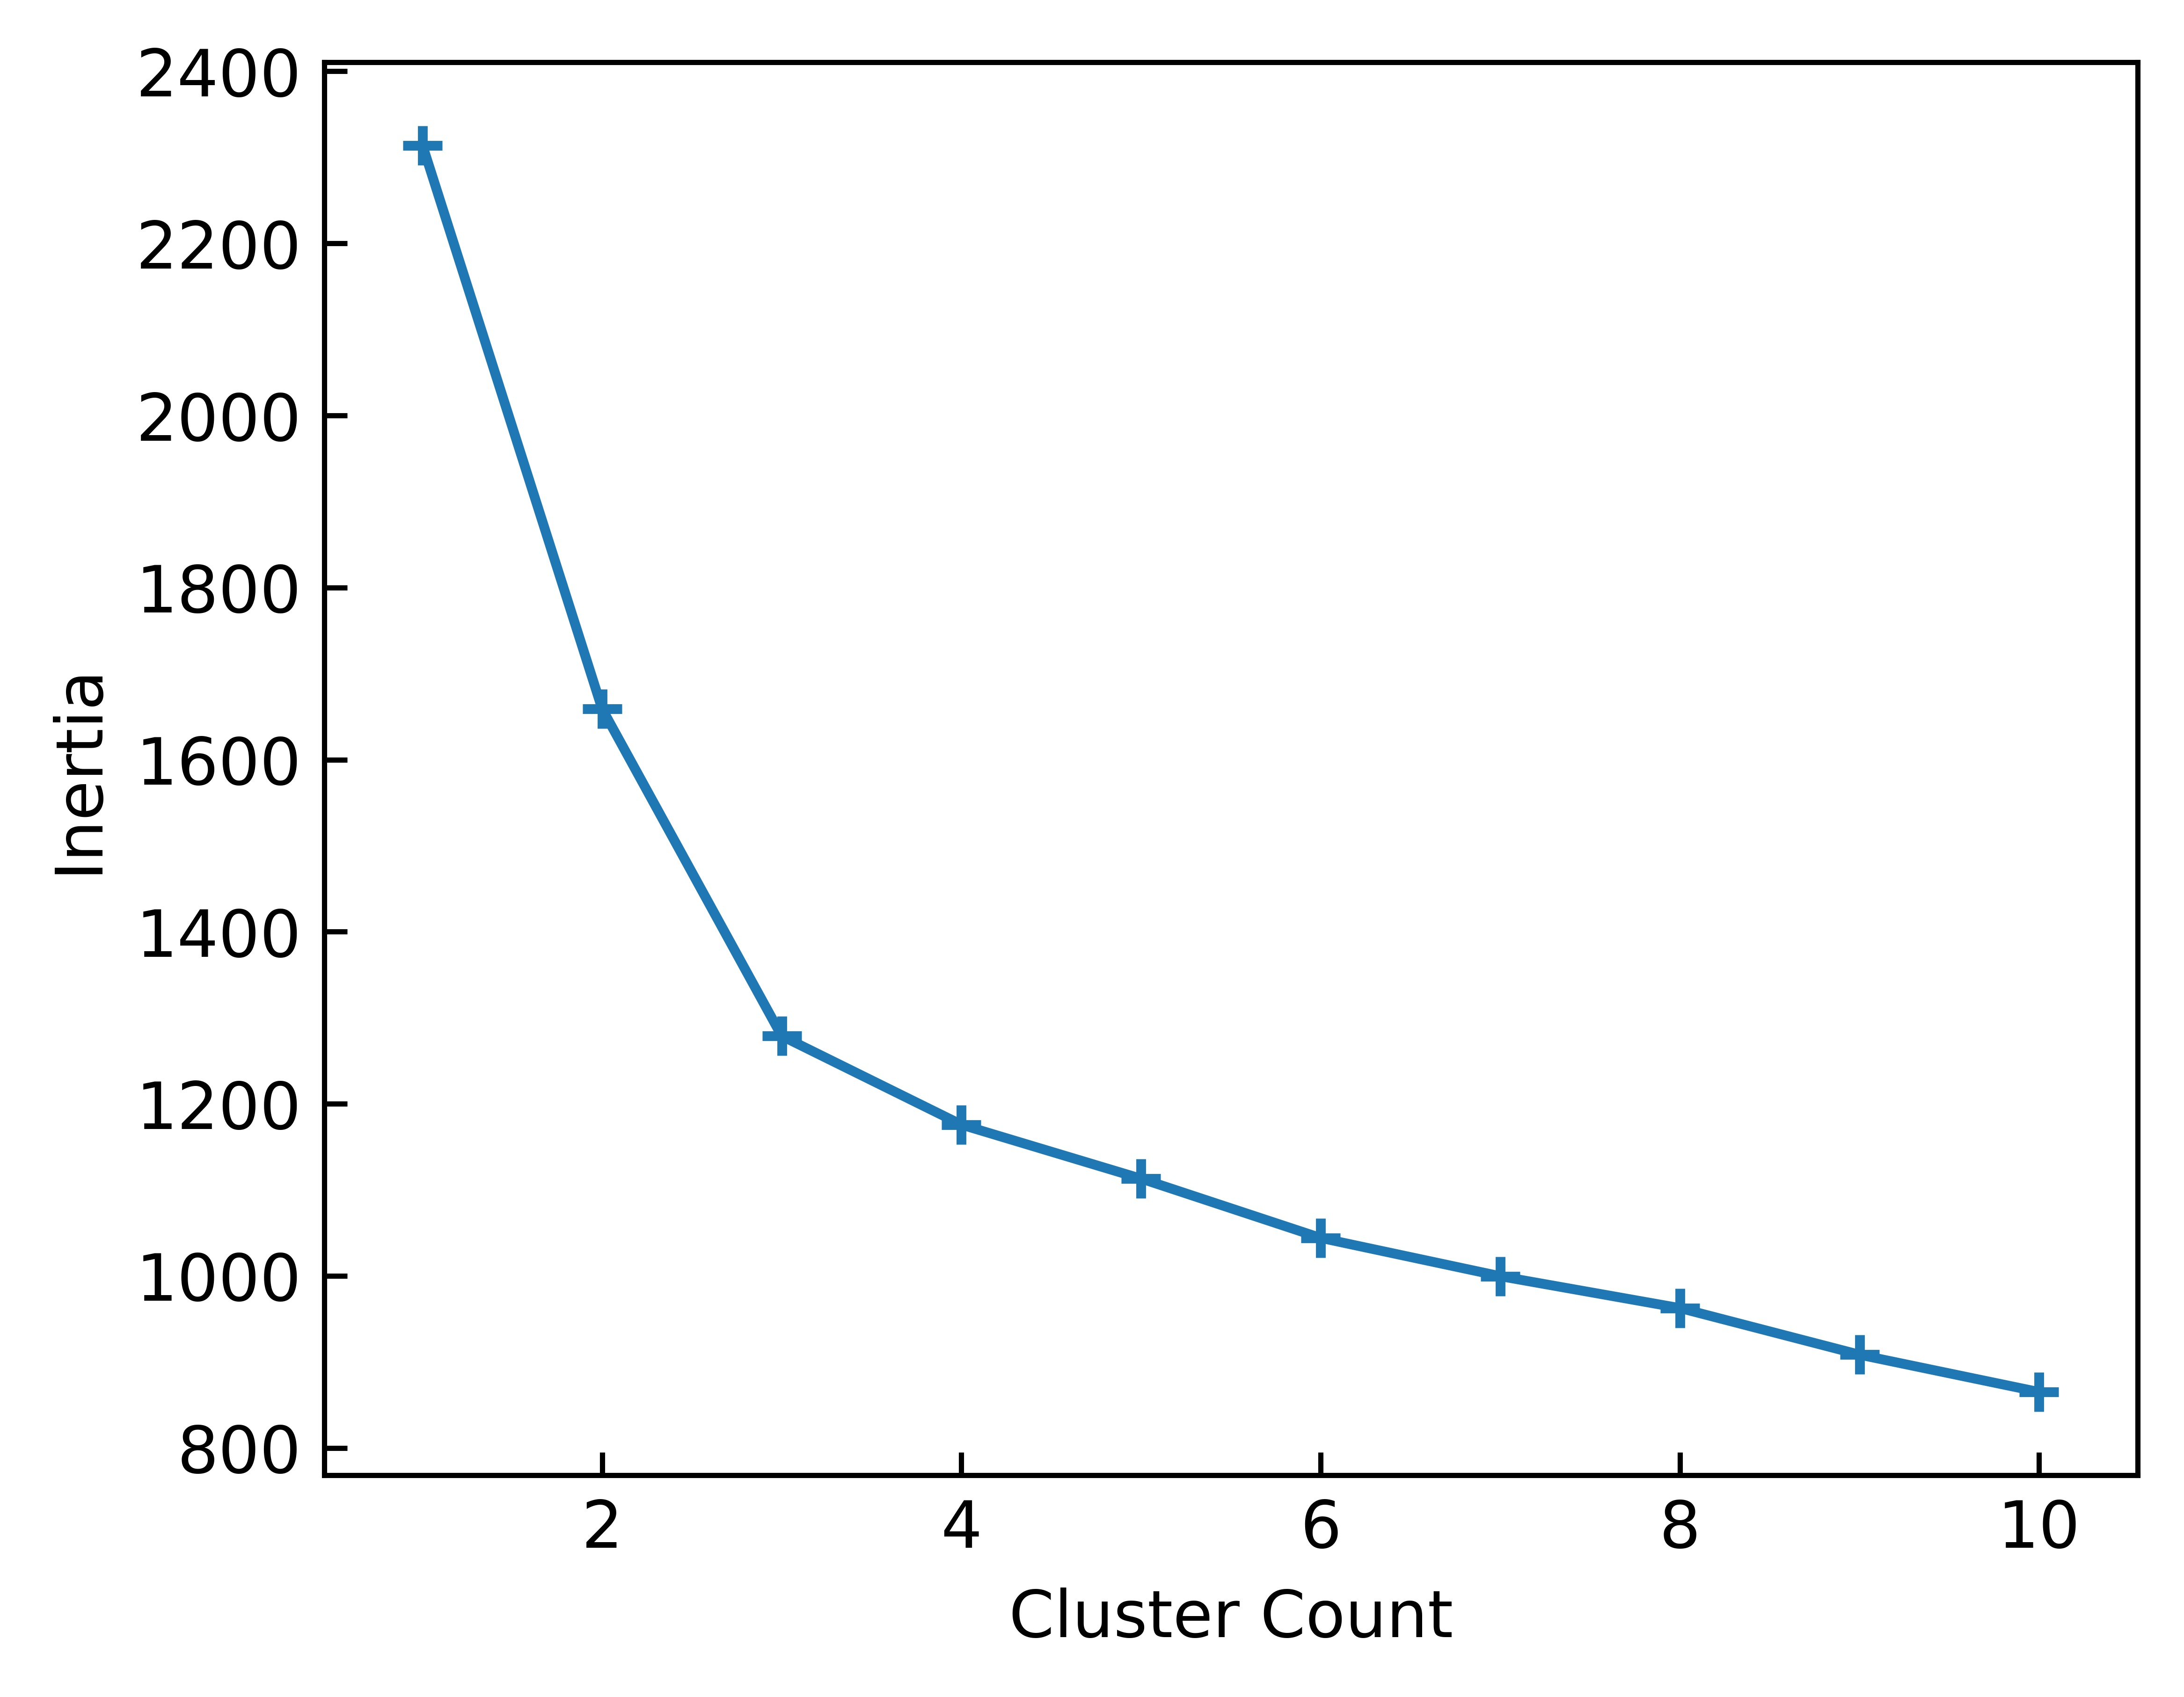
\includegraphics[width=0.65\textwidth]{1.jpg}
	\bicaption{$W_{k}\sim k$曲线}{$W_{k}\sim k$ Curve}
\end{figure}
\par 

根据\textbf{图1},可见$k=3$为曲线从迅速下降到平缓下降的拐点,即“手肘”的位置,故选取$k=3$作为最优簇数$k$。这一结果与wine数据集的样本类数是一致的。
\subsubsection{轮廓系数(Silhouette Coefficient)方法}
实验代码运行时长为1.26 s。作出$s\sim k$曲线,如\textbf{图2}所示。\par 
\begin{figure}[h]
	\centering
	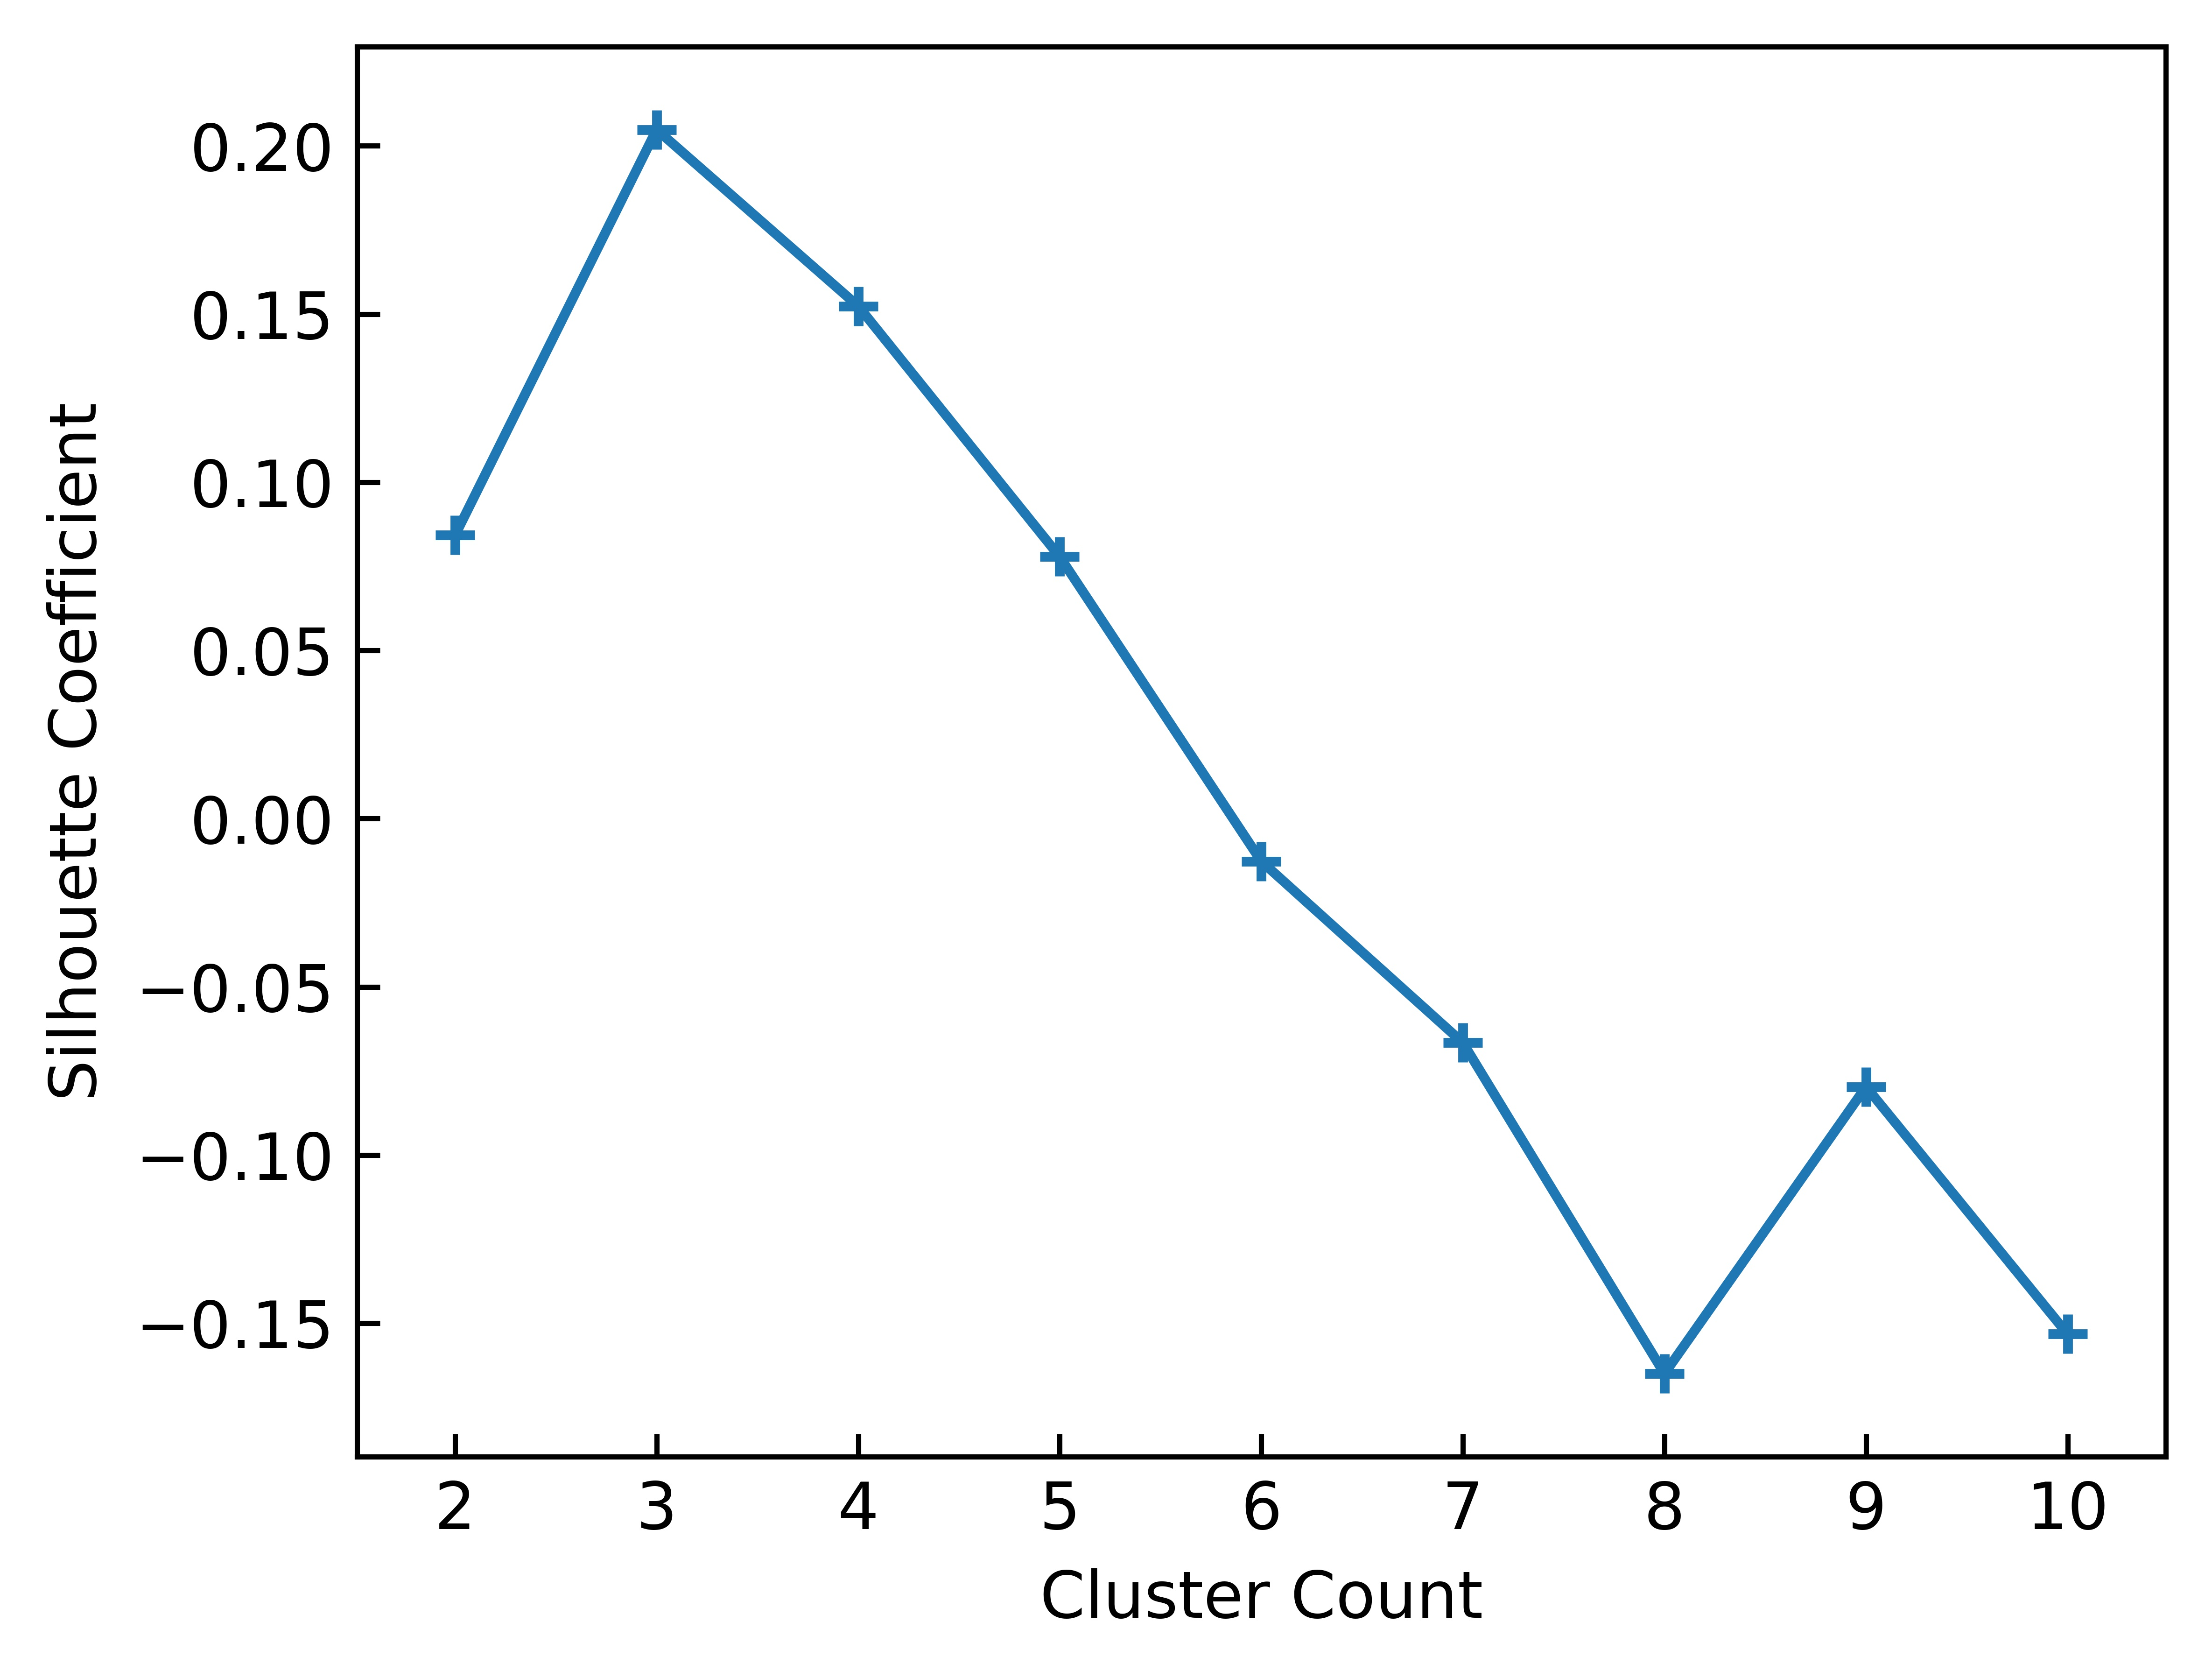
\includegraphics[width=0.65\textwidth]{2.jpg}
	\bicaption{$s\sim k$曲线}{$s\sim k$ Curve}
\end{figure}
\par 
根据\textbf{图2},可见$k=3$时$s$取最大值,故选取$k=3$作为最优簇数$k$。这一结果与wine数据集的样本类数是一致的。

\subsubsection{间隔统计量(Gap Statistic)方法}
首先计算不同$k$值下的${\rm Gap}(k)$,实验代码运行时长为14.2 s。作出${\rm Gap}(k)\sim k$曲线,如\textbf{图3}所示。\par 
根据\textbf{图3},可见$k=1$时${\rm Gap}(k)$取最大值,根据间隔统计量方法的原理,应当选取$k=1$作为最优簇数$k$。这一结果与wine数据集的样本类数不一致。\par 
进一步地,计算不同$k$值下的${\rm Diff}(k)$,实验代码运行时长为8.78 s。作出${\rm Diff}(k)\sim k$曲线,如\textbf{图4}所示。\par 
\begin{figure}[htbp]
	\centering
	\begin{minipage}[t]{0.49\textwidth}
		\centering
		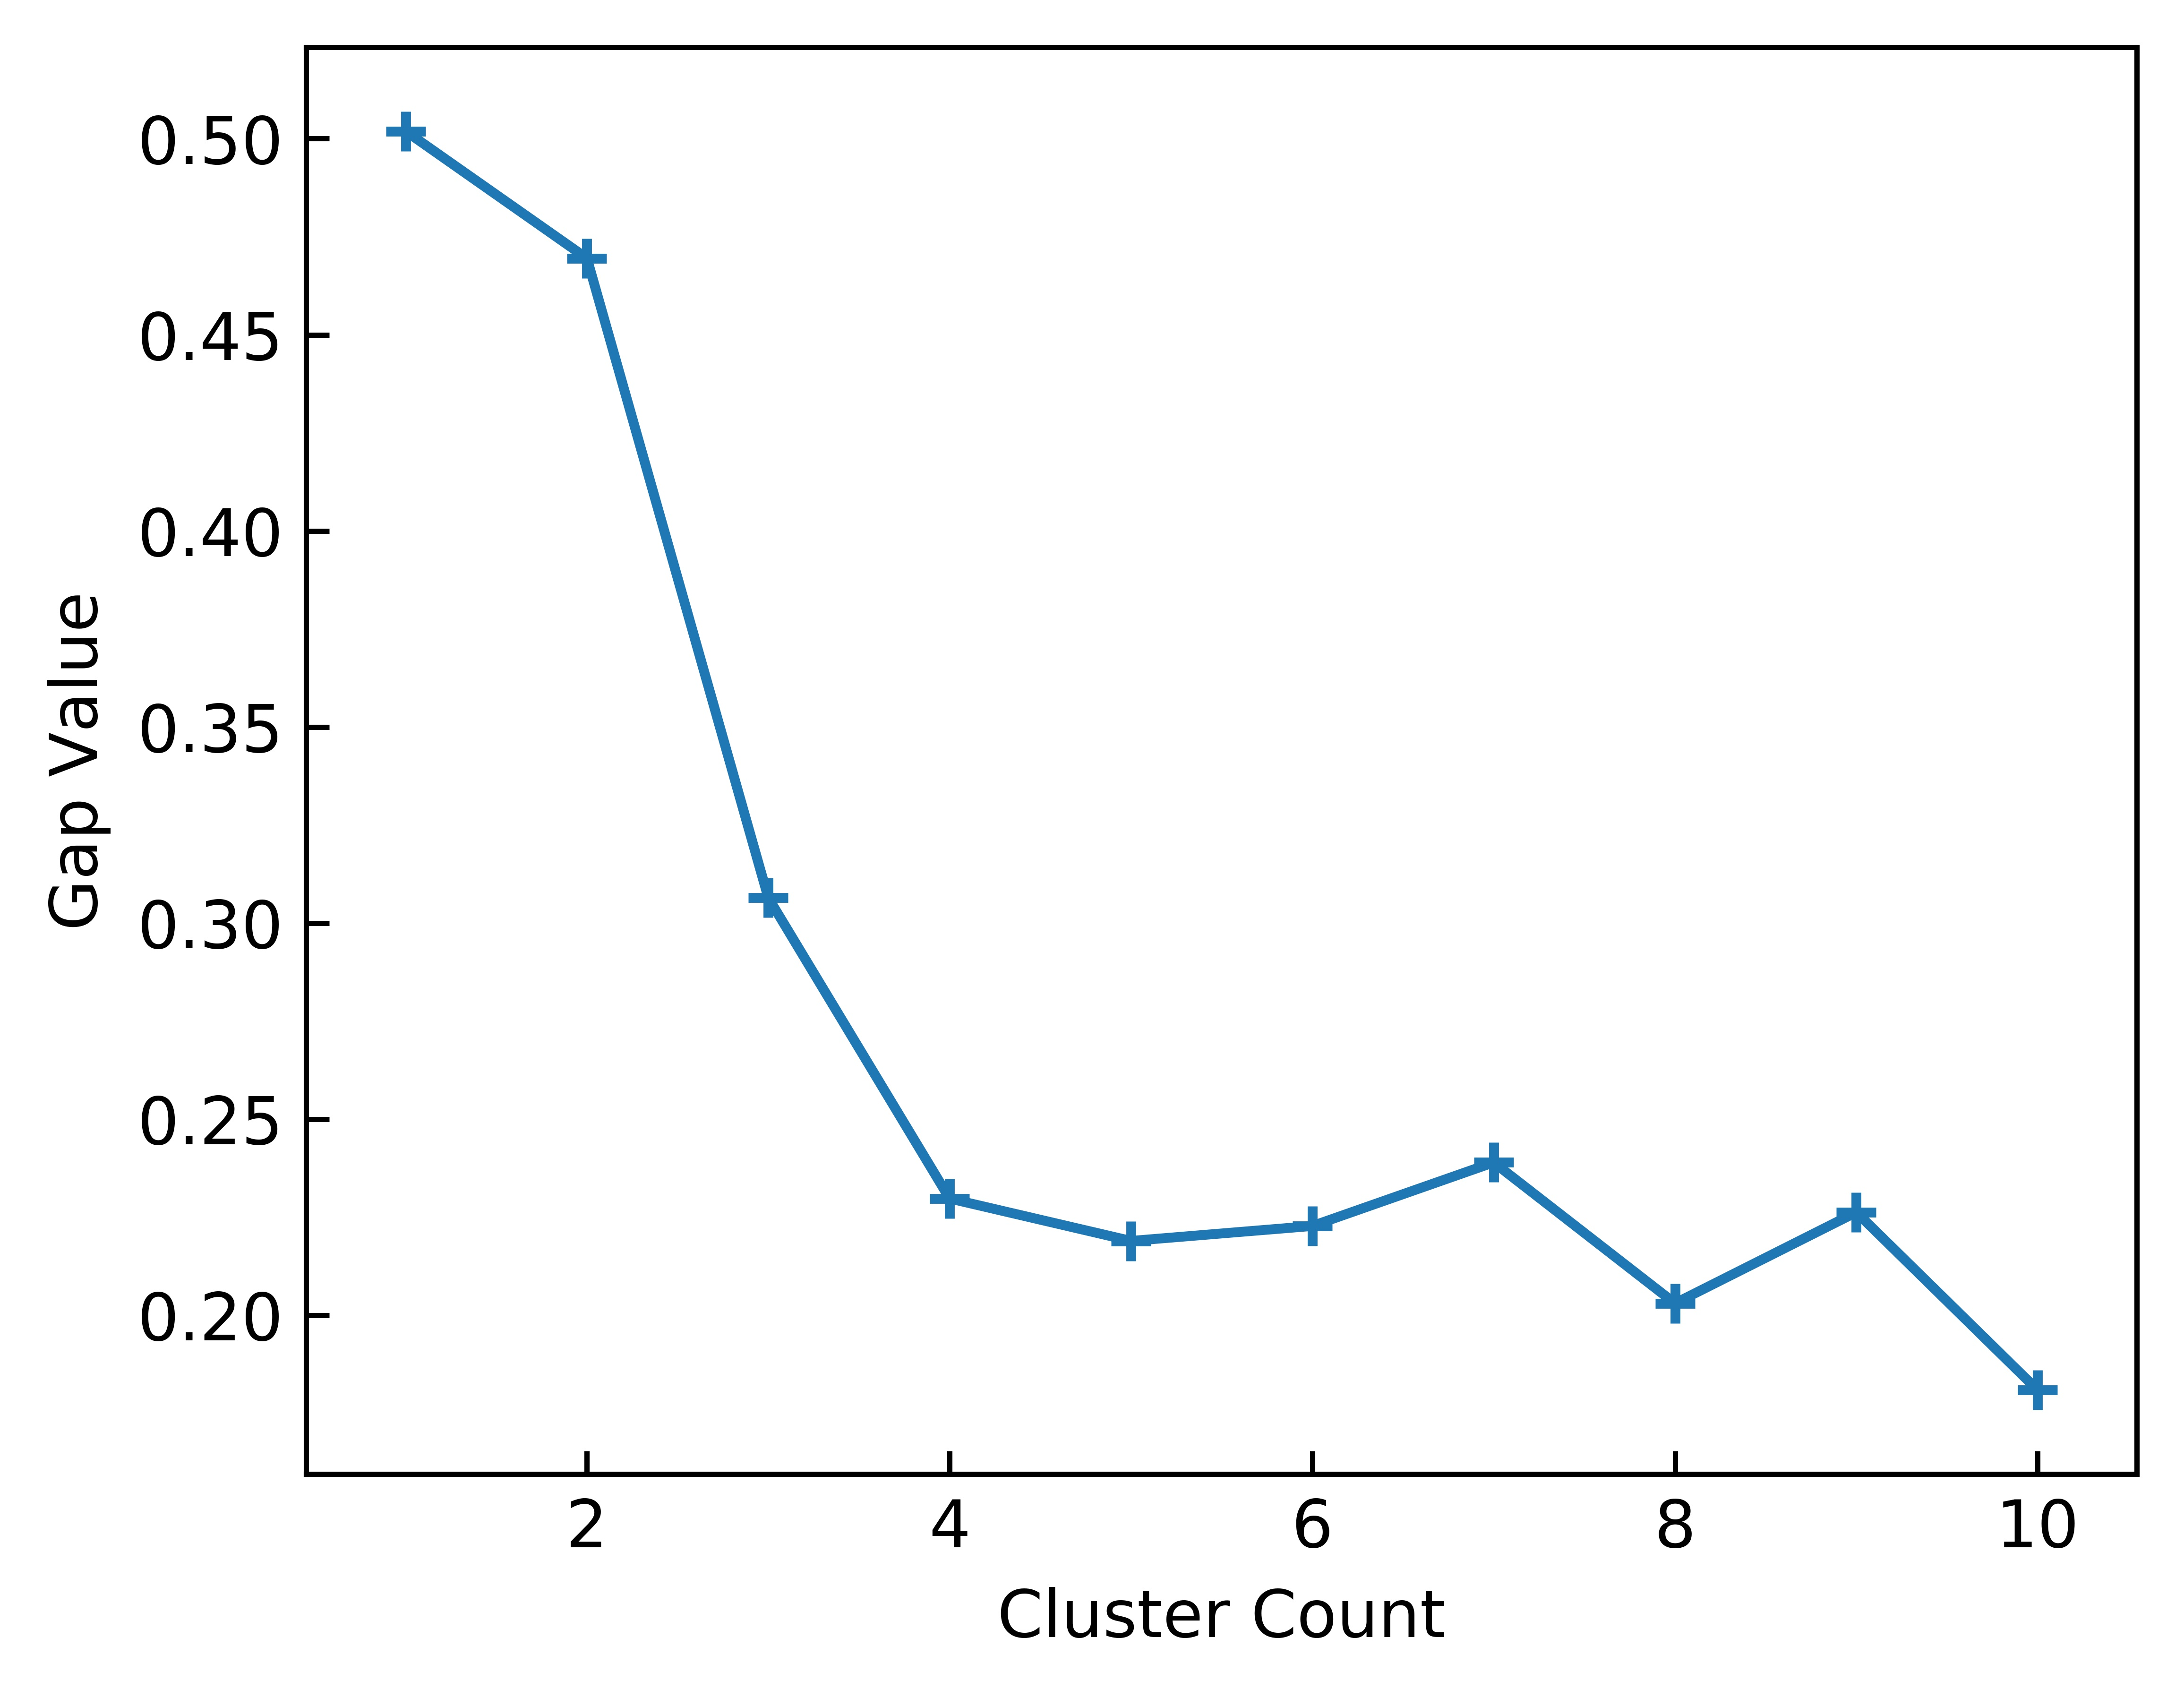
\includegraphics[width=1\textwidth]{3.jpg}
		\bicaption{${\rm Gap}(k)\sim k$曲线}{${\rm Gap}(k)\sim k$ Curve}
	\end{minipage}
	\begin{minipage}[t]{0.49\textwidth}
		\centering
		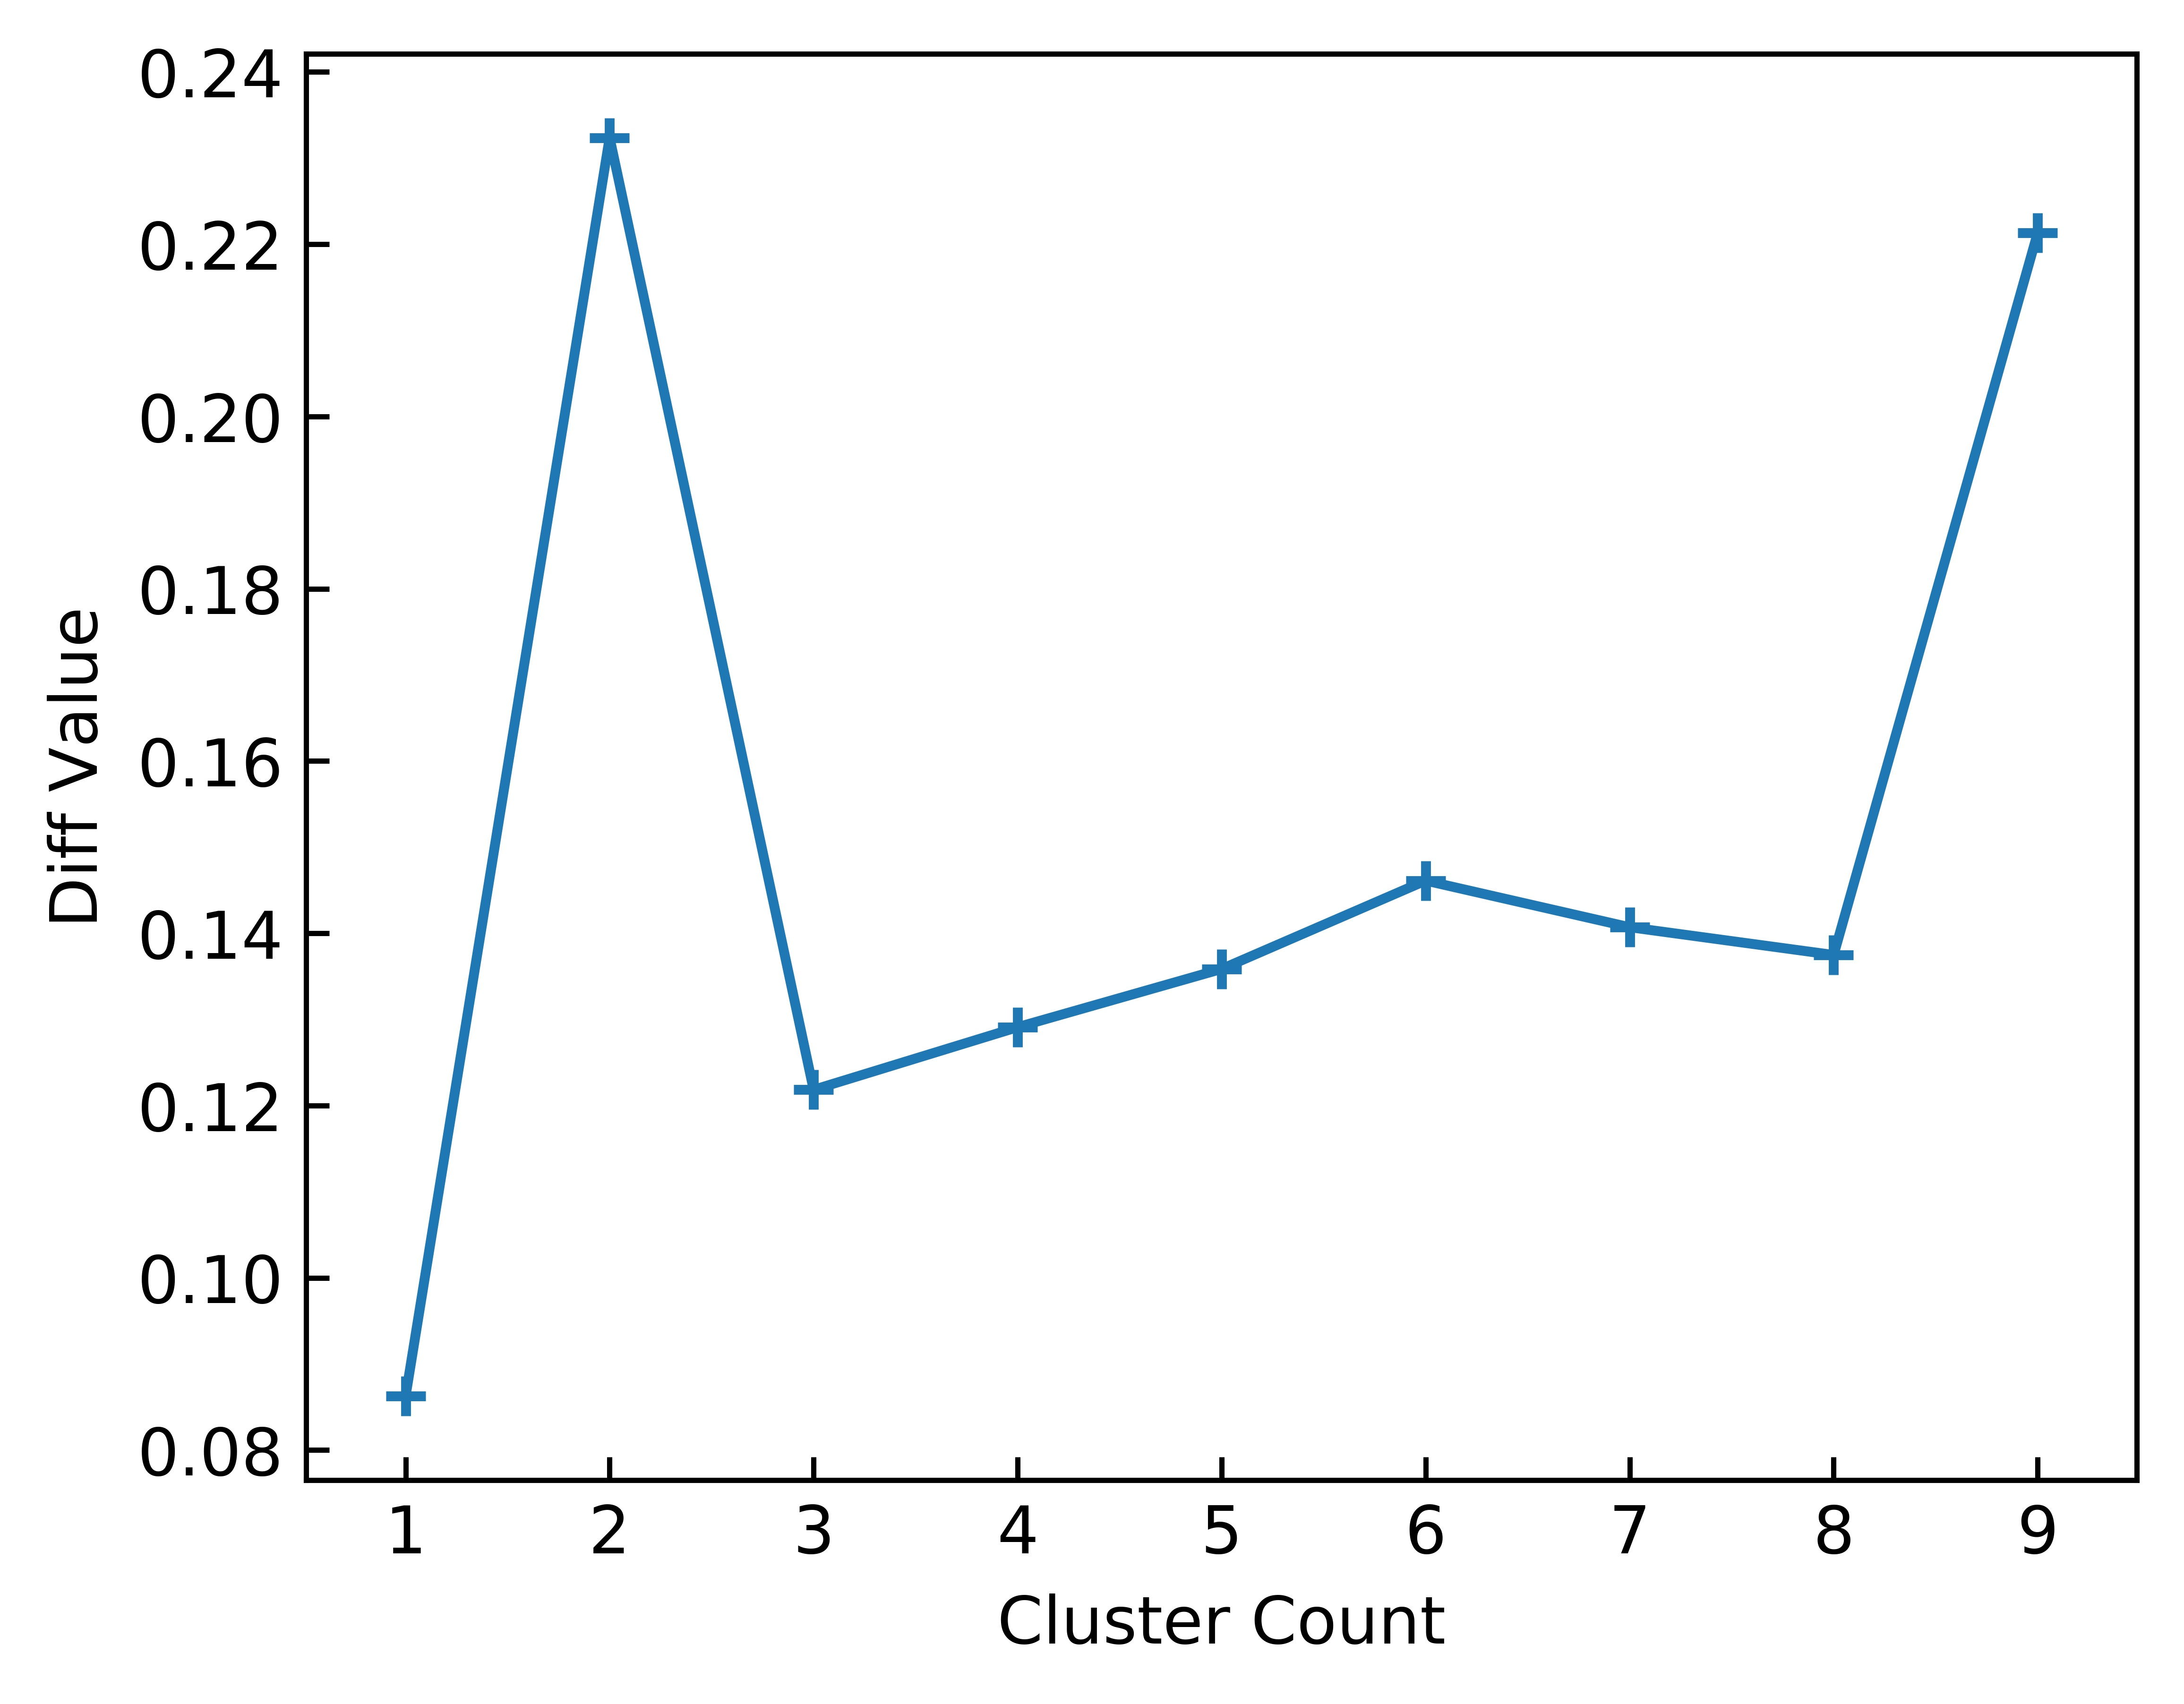
\includegraphics[width=1\textwidth]{4.jpg}
		\bicaption{${\rm Diff}(k)\sim k$曲线}{${\rm Diff}(k)\sim k$ Curve}
	\end{minipage}
\end{figure}
\par
根据\textbf{图4},可见恒有${\rm Diff}(k)\geq 0$,根据间隔统计量方法的原理,应当选取$k=1$作为最优簇数$k$。这一结果与wine数据集的样本类数不一致。

\subsection{结果分析}
根据2.5的实验结果,手肘法(Elbow Method)和轮廓系数(Silhouette Coefficient)方法确定最优簇数$k=3$,与wine数据集的样本类数一致。而间隔统计量(Gap Statistic)方法确定最优簇数$k=1$,与wine数据集的样本类数不一致,其原因可能是wine数据集的样本数量较少,间隔统计量方法计算结果波动较大,从而导致对最优簇数$k$的判断出现偏差。\par 
对于需要预先设定簇数$k$的聚类算法,若无法事先根据实际需要确定最优簇数$k$,则在确定最优簇数$k$时可以综合考虑手肘法(Elbow Method)、轮廓系数(Silhouette Coefficient)方法、间隔统计量(Gap Statistic)等方法所给出的结果,结合实际需要作出综合判断。

   

\vbox{}

\bibliographystyle{ieeetr}
\bibliography{b}



\end{document}